\section{Introduction}
\label{sec:intrp}

%Purpose
%- what is the micro:bit?
% http://www.bbc.co.uk/programmes/articles/4hVG2Br1W1LKCmw8nSm9WnQ/the-bbc-micro-bit

The micro:bit is a small programmable and embeddable computer designed, 
developed and deployed by the BBC and partners (including Microsoft, 
and Lancaster University) to approximately 800,000 UK middle school students
in 2015-2016. Part of the BBC's Make it Digital Campaign, the BBC described the
micro:bit as its ``most ambitious education initiative in 30 years, 
with an ambition to inspire digital creativity and 
develop a new generation of tech pioneers.''~\cite{BBCwebsite}

% reference the competition and show what's different (hardware)
% https://barrettsprojects.wordpress.com/2012/09/15/tap-and-double-tap/ 


Figure~\ref{fig:microbit} shows (a) the front and (b) the back of the
micro:bit, which measures 4x5 centimeters. Like the Arduino Uno,
the micro:bit is a single-board microcontroller that can be programmed
via a host computer (usually a laptop or desktop)
and then embedded in projects where it runs on battery power.
In contrast to the Uno, which has no built-in sensors, the micro:bit 
board hosts a variety of sensors (temperature, accelerometer, compass, light level), 
a 5x5 LED matrix, two user-defined buttons, as well as Bluetooth
Low Energy (BLE) communications.

The design of the micro:bit hardware was driven by the
first two objectives of the micro:bit project:
(1) to provide a simple creative experience for physical computing, wearable and Internet of Things (IoT) projects;
(2) to supply a device that can continue to provide learning opportunities as the user's expertise grows.

On the hardware side, the micro:bit's built-in sensors, buttons and LED display 
allow many projects to be completed with no additional hardware or wiring. 
The holes on micro:bit's edge
connector allows additional external sensors and actuators to be connected via crocodile clips.
As with Arduino, an ecosytem of micro:bit shields that the micro:bit can plug into expand
its capabilities greatly. The micro:bit's BLE capabilities introduces networking to the
picture, and enables streaming of data and command/control operations among the micro:bit, 
smartphones, laptops, as well as other micro:bits.

\begin{figure} 
\begin{tabular}{cc}
  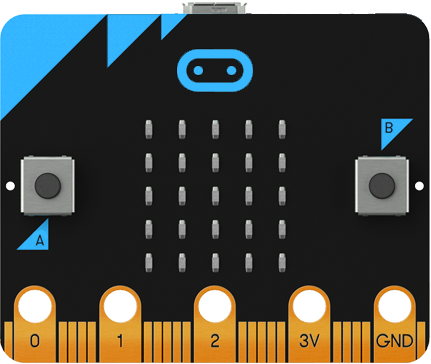
\includegraphics[width=1.5in]{images/microbit-front.png} &
  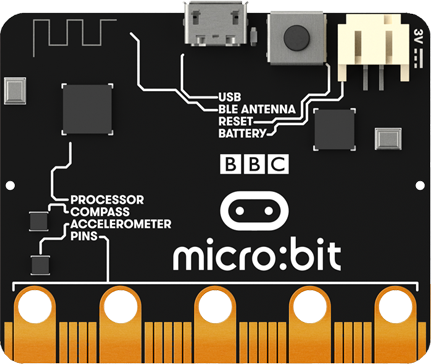
\includegraphics[width=1.5in]{images/microbit-back.png} \\
  (a) & (b) 
\end{tabular}
\caption{\label{fig:microbit}The micro:bit: (a) front, with two buttons, 
  5x5 LED display, and edge connector (bottom); (b) back, with processor, accelerometer, compass, Bluetooth, USB and battery ports.}
\end{figure}

% micro:bit is an embeddable, reactive, networked computing system

The design of the micro:bit firmware and coding tools also were oriented towards a 
simple starting experience with room for progression. In particular, the coding 
objectives of the project were: (3)
to give students an exciting, engaging introduction to coding;
(4) to stimulate curiosity about how computing technologies can be utilized 
  to solve problems that students identify. 

[info about the coding solution: BBC identified using a web app and C/C++ compiler in the cloud
to create a binary executable that would then be flashed onto micro:bit;
final design put the entire toolchain in web app, without need to invoke C/C++ compiler to
compile the user's program; ARM DAPlink solution makes micro:bit appear as USB pen drive
on all operating systems; MicroPython provided second programming solution with entire toolchain
on the micro:bit!!]

% fast forwarding:
%
%- BBC micro:bit designed/implemented by set of partners (2015-2016)
%- UK focused (philanthropic effort with partners contributing time, people, cash)

What happened:
\begin{itemize}
\item implementation and rollout took half a year longer than expected (surprise, with devices landing
in classrooms in February of 2016, more than halfway through the 2015-2016 school year in UK);
\item first full school year was 2016-2017, during which micro:bit Education Foundation got
started; 
\item now have two full school years complete with experience in more countries 
\item lots of partners participating (ICSTE and CSTA 2018)!!
\end{itemize}


%- A lot of lessons learned from delivering end-to-end experience in UK and other countries
%   - hardware (unique design, as already mentioned)
%   - firmware:  high-level C/C++ runtime and ARM's DAPlink
%   - web-based IDE: no C/C++ compiler needed to compile user code
%   - content
%   - training
% In country partnerships

% success of micro:bit due to 
% - Low-cost, simplicity
% - Partnerships (hardware, software, content, training)
% - Platform???
% - 

% - why is it interesting?
%   - edge/physical/IoT computing
%   - build off of Scratch/Blockly, but untethered (via in-browser compiler)
%   - transition to JavaScript and Python

% - BBC rollout in UK
% - Global reach
%    - BBC rollout mirrored in other countries
%    - Communities
%      - Sri Lanka user group: http://microbitslug.org/
%      - UK libraries (loan program)
%    - third party editors

% Design considerations (technical requirements, steal from LCTES paper)

%   - hardware clearly distinguished from Arduino
%     - no wiring required to do interesting things (integrated sensors and outputs, etc.)
%     - device appears as USB pen drive (drag-and-drop programming)
 
%   - As with Arduino, embedding device into projects is essential (from beginner to maker)
%     - battery power
%     - works disconnected from host
%     - wearable, transportable
%     - low cost
%     - edge connector for easy connection to "shields"

%   - support for scripting languages (JavaScript and Python; no C/C++ for beginners)
%     - event-based programming model

%   - web-based IDE
%     - no apps or device drivers to install
%     - school considerations (minimize IT admin involvement)

%   - layered approach
%     - simple for absolute beginners to get started
%     - room for students to advance to more complex projects

% - worldwide rollout
%   - microbit.org, makecode.microbit.org

% from http://cacm.acm.org/system/assets/0000/6052/CACM_Author-Guidelines.pdf 

% 2.3.4 Contributed Articles
% Contributed Articles cover the wide and abundant spectrum of the computing field—its open challenges, 
% technical visions and perspectives, educational aspects, societal impact, significant applications and 
% research results of high significance and broad interest. 

% we have:
% + technical vision
% + educational aspect and societal impact
% + signification application
% - research results of high significance and broad interest: see LCTES 2018 article

% Topics covered must reach out to a very broad technical audience.
% Articles in Communications should be aimed at the broad computing and information technology community.

% A Contributed Article should set the background and provide introductory references, 

% define fundamental concepts, 

% compare alternate approaches, 

% Arduino
% Scratch (tethered)
% MicroPython

% and explain the significance or application of a particular technology 

% or result by means of well-reasoned text and pertinent graphical material. 

% The use of sidebars to illustrate significant points is encouraged.

% Full-length Contributed Articles should consist of up to 4,000 words, 
% contain no more than 25 references, 3-4 tables, 3-4 figures, 
% and be submitted to: http://cacm.acm.org/submissions.

% Submissions to the Contributed Articles section should be accompanied by a cover letter indicating:
% • Title and the central theme of the article; 
% • Statement addressing why the material is important to the computing field and of value to the Communications reader;
% • Names and email addresses of three or more recognized experts who would be considered appropriate to review the submission.


% from the BBC RFP

% Make it Digital is a BBC initiative to inspire a new generation to get creative with 
% coding, programming and digital technology. With a major focus in 2015, Make it Digital 
% will help all audiences see how Britain has helped shape the digital world, why digital 
% skills matter and their growing importance to our future. For younger audiences, Make it 
% Digital will help them discover the world of digital, see their creative potential in it 
% and inspire them to take their first steps in computational thinking and digital skills. 

% In September/October [2015], as part of the overall Make It Digital project, BBC Learning aims 
% to give away one million small, programmable, wearable devices. The device can be used 
% in classrooms and the home to create an engaging hands-­‐on learning experience that 
% allows any level of coder from absolute beginner to advanced maker to get involved and 
% be part of something exciting. Approximately 800,000 devices will go to every child in 
% the UK at Year 7 (tbc) and a further 200,000 will be made available to distribute 
% through competitions and other activities targeting other groups covering both children 
% and adults. 

% We anticipate that an online coding site will support the devices. The site will allow 
% owners to create programmes to run on their own devices and/or share programmes and code 
% with others. 










